%!TEX root = ../thesis.tex
%*******************************************************************************
%****************************** Third Chapter **********************************
%*******************************************************************************

\chapter{Results}

% **************************** Define Graphics Path **************************
\ifpdf
    \graphicspath{{Chapter3/Figs/Raster/}{Chapter3/Figs/PDF/}{Chapter3/Figs/}}
\else
    \graphicspath{{Chapter3/Figs/Vector/}{Chapter3/Figs/}}
\fi

% Oscillations 
\section{Regulation of the CLV3 domain induces periodicity when perturbed}
When tracking the number of CLV3 nuclei identified by Costanza, the results
observable in \cref{fig:clv3_trajs} shows the number of observed CLV3 nuclei
increasing for plants 2, 4, 13, and 15, corresponding to a visually observable
enlargement of the CLV3 domain in \FIG (timelapse of example plant over 4
timepoints?). Similarly, fluctuations in this number can be seen not to 
correlate with the mean expression as described in
\cref{tab:corr_nNucl_meanExpr}. % and therefore ought to be structural

\begin{figure}[H]
  \centering
  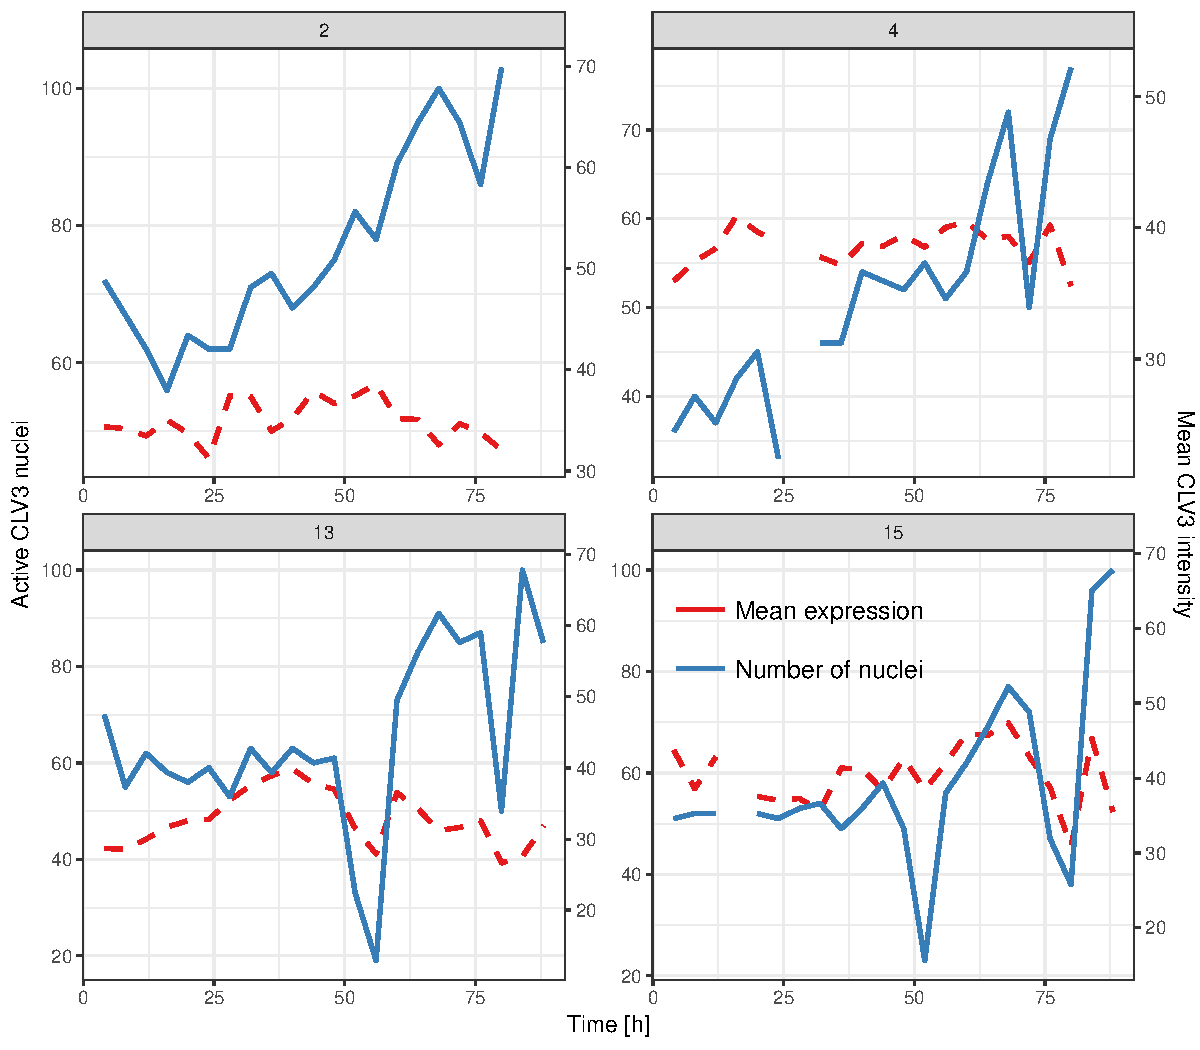
\includegraphics[width=.8\textwidth]{clv3nucl_trajectories.pdf}
  \caption{Add caption}
  \label{fig:clv3_trajs}
\end{figure}

\begin{table}
  \centering
  \caption{TODO}
  \label{tab:corr_nNucl_meanExpr}
  \begin{tabular}{ll}  \toprule
    Plant & p-value \\ \midrule
    2     & 0.48    \\
    4     & 0.84    \\
    13    & 0.91    \\
    15    & 0.11    \\ \midrule
    All   & 0.50    \\ \bottomrule
  \end{tabular}
\end{table}

In order to assess the extent of the fluctuations the lines were detrended using
a second order Loess fit to each curve. When performing a continuous time
Fourier transform in order to extract amplified modes, the plants have are
biased towards the fourth mode in each respective transformation, as depicted in
\cref{fig:modes}, which corresponds to periodicity of $\sim$16~hours. \FIG
\todo{map this to light / dark hour cycles?}
% and are hence not circadian

In addition to this periodicity, the number of nuclei identified correlates
positively with the number of division events observed in each timepoint for
three out of the four plants (\cref{fig:corr_nNucl_nDivs}. Plant 13, like in 
\cref{fig:clv3_trajs} is the one anomously behaving specimen.
\unsure{Should I add other correlations and just draw plots?}

\begin{figure}[H]
  \centering
  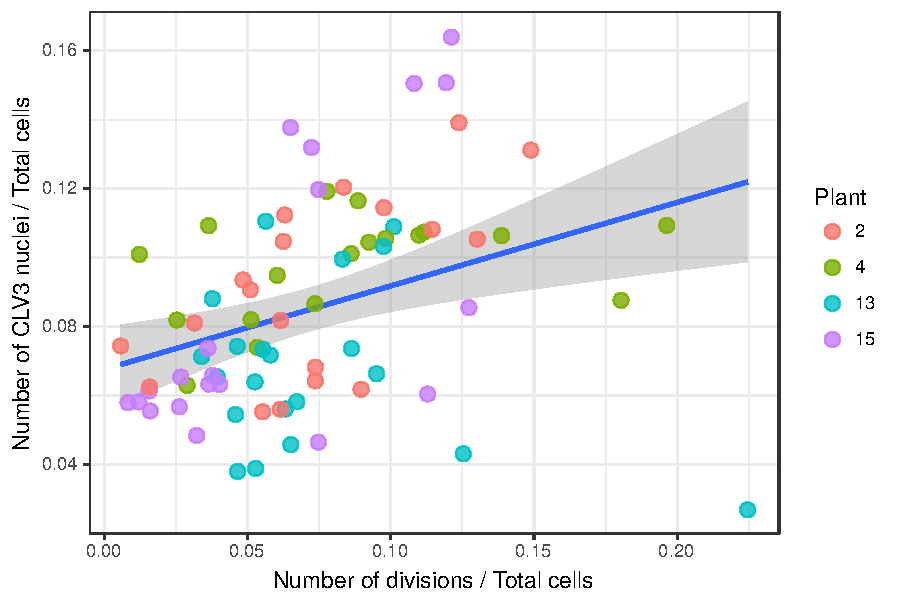
\includegraphics[width=.8\textwidth]{corr_nNucl_nDivs.pdf}
  \caption{Add caption}
  \label{fig:corr_nNucl_nDivs}
\end{figure}

% Trajectories
% Fourier analysis

\section{Distribution shifting suggests epidermal regulation}
\subsection{CLV3 is induced in the epidermis}
A layer-wise separation of the CLV3 expression can be seen in particular between
\Lone and \Ltwo, as visualised in \cref{fig:clv3_layer_sep}. 

\begin{figure}[H]
  \centering
  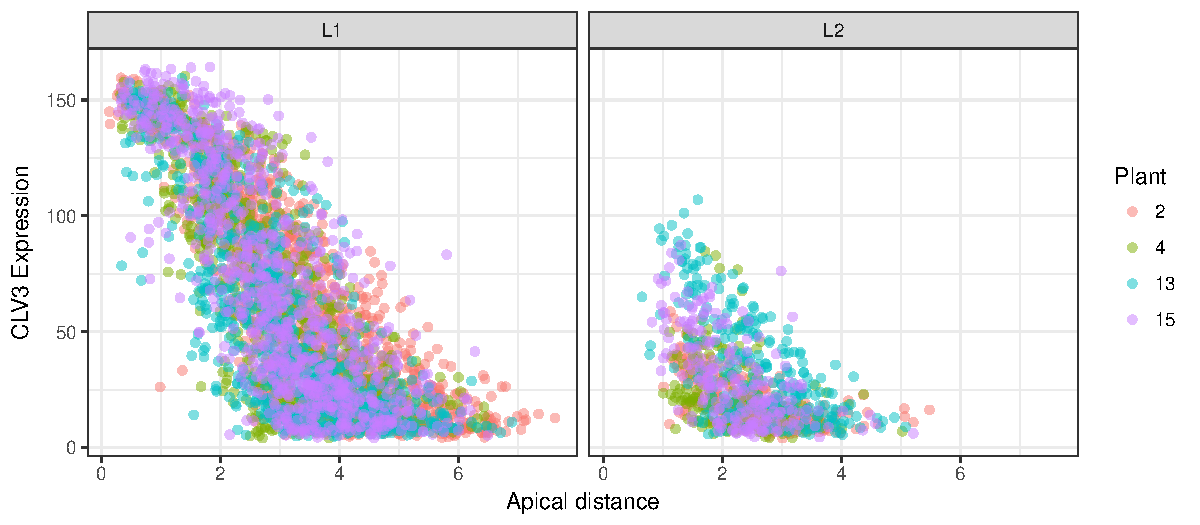
\includegraphics[width=.8\textwidth]{clv3_layer_sep.pdf}
  \caption{Add caption}
  \label{fig:corr_nNucl_nDivs}
\end{figure}

% Support this with simple model?

\subsection{Low variance in CZ indicates tight regulation at apex}
% This holds regardless of what distribution looks like

\section{Cell lineage tracking implies dsRED technical artefacts}
Just show lineages or quantify behaviour? \\

TODO: Justification for decay. Assume movement out of CZ proportional to
division rate $k_{div}$, such that $\dot{R} \propto k_{div}$. We thus have
$R = kt$. Assume linear degradation of CLV3 such that $\dot{C} = -k_{deg} =
\frac{\dd C}{\dd t} = \frac{\dd C}{\dd R} \frac{\dd R}{\dd t}$. We therefore have
$\frac{\dd C}{\dd R} = \frac{\dd C}{\dd t} = -\frac{k_{deg}}{k_{div}}$. Justify
decay rate observed in trajectories or smth like that?

\section{Deep-tissue cells divide at a slower rate}
Still unknown.
